\documentclass[tikz,border=20pt]{standalone}
\usetikzlibrary{calc,arrows.meta,decorations.pathmorphing}
\usepackage{xcolor}

\definecolor{nightdark}{HTML}{030712}
\definecolor{nightblue}{HTML}{0F172A}
\definecolor{lanternorange}{HTML}{EA580C}
\definecolor{goldfire}{HTML}{FBBF24}
\definecolor{cyanfire}{HTML}{38BDF8}
\definecolor{pinkfire}{HTML}{F472B6}

\begin{document}
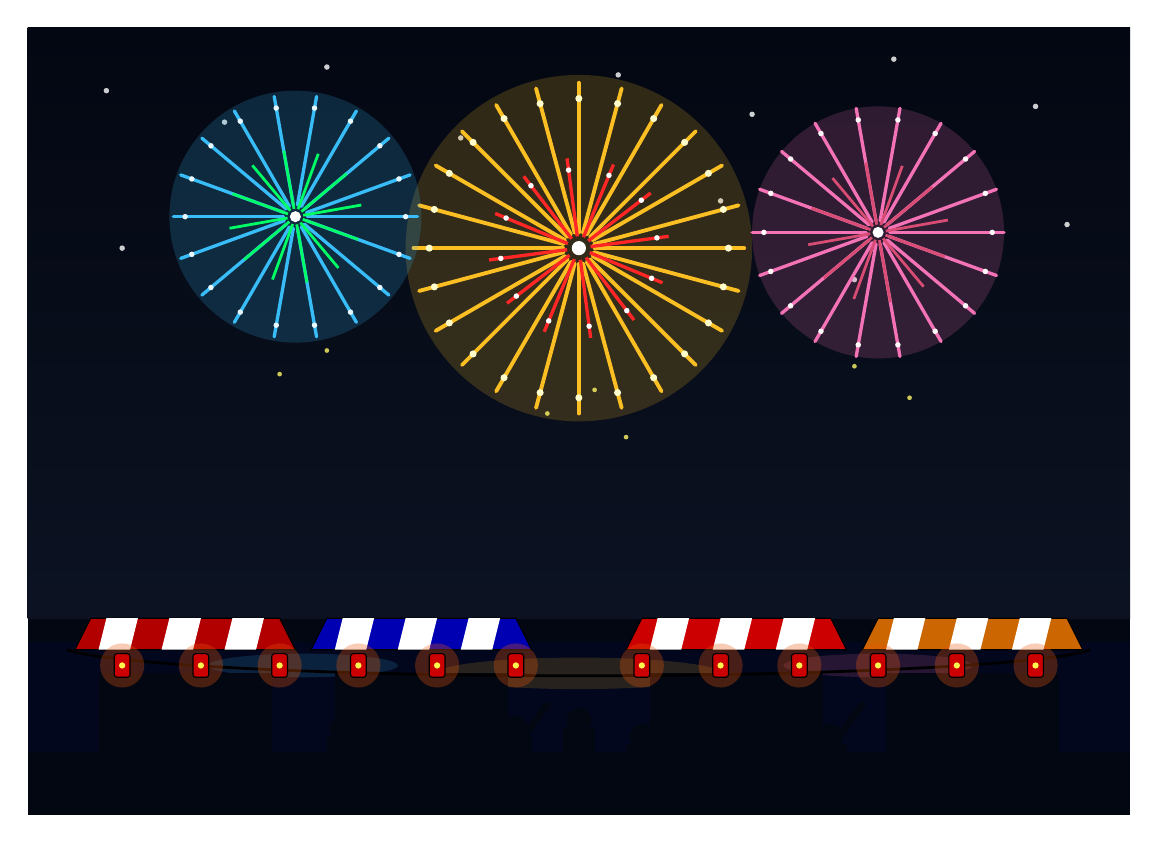
\begin{tikzpicture}[x=1cm, y=1cm]

  % Deep Night Sky Canvas
  \fill[nightdark] (-7, -5) rectangle (7, 5);
  \shade[top color=nightdark, bottom color=nightblue!80!black] (-7, -2.5) rectangle (7, 5);

  % Scattered Stars
  \foreach \pos in {(-6, 4.2), (-4.5, 3.8), (-3.2, 4.5), (-1.5, 3.6), (0.5, 4.4), (2.2, 3.9), (4.0, 4.6), (5.8, 4.0), (6.2, 2.5), (-5.8, 2.2), (1.8, 2.8), (3.5, 1.8)} {
    \fill[white, opacity=0.8] \pos circle (0.035);
  }

  % Water / River Surface (Bottom: -5 to -2.8)
  \fill[nightdark!95!blue] (-7, -5) rectangle (7, -2.8);
  % Water reflections
  \fill[goldfire, opacity=0.15] (0, -3.2) ellipse (1.8 and 0.2);
  \fill[cyanfire, opacity=0.15] (-3.5, -3.1) ellipse (1.2 and 0.15);
  \fill[pinkfire, opacity=0.15] (3.8, -3.1) ellipse (1.2 and 0.15);

  % ==================== 1. FIREWORK BURSTS ====================
  % Center Gold/Crimson Burst (at (0, 2.2))
  \fill[goldfire, opacity=0.18] (0, 2.2) circle (2.2);
  \foreach \a in {0, 15, ..., 345} {
    \draw[goldfire, line width=1.4pt, line cap=round]
      (0, 2.2) ++(\a:0.2) -- ++(\a:1.9);
    \fill[yellow!20] (0, 2.2) ++(\a:1.9) circle (0.045);
  }
  % Inner crimson core
  \foreach \a in {7.5, 37.5, ..., 337.5} {
    \draw[red!80!pink, line width=1.2pt]
      (0, 2.2) ++(\a:0.15) -- ++(\a:1.0);
    \fill[white] (0, 2.2) ++(\a:1.0) circle (0.035);
  }
  \fill[white] (0, 2.2) circle (0.09);

  % Left Cyan & Emerald Burst (at (-3.6, 2.6))
  \fill[cyanfire, opacity=0.18] (-3.6, 2.6) circle (1.6);
  \foreach \a in {0, 20, ..., 340} {
    \draw[cyanfire, line width=1.2pt, line cap=round]
      (-3.6, 2.6) ++(\a:0.15) -- ++(\a:1.4);
    \fill[cyan!10] (-3.6, 2.6) ++(\a:1.4) circle (0.035);
  }
  \foreach \a in {10, 40, ..., 340} {
    \draw[green!60!cyan, line width=1pt]
      (-3.6, 2.6) ++(\a:0.1) -- ++(\a:0.75);
  }
  \fill[white] (-3.6, 2.6) circle (0.07);

  % Right Pink & Purple Burst (at (3.8, 2.4))
  \fill[pinkfire, opacity=0.18] (3.8, 2.4) circle (1.6);
  \foreach \a in {0, 20, ..., 340} {
    \draw[pinkfire, line width=1.2pt, line cap=round]
      (3.8, 2.4) ++(\a:0.15) -- ++(\a:1.45);
    \fill[pink!10] (3.8, 2.4) ++(\a:1.45) circle (0.035);
  }
  \foreach \a in {10, 40, ..., 340} {
    \draw[purple!60!pink, line width=1pt]
      (3.8, 2.4) ++(\a:0.1) -- ++(\a:0.8);
  }
  \fill[white] (3.8, 2.4) circle (0.07);

  % Falling Sparkles
  \foreach \pos in {(0.2, 0.4), (-0.4, 0.1), (0.6, -0.2), (-3.2, 0.9), (-3.8, 0.6), (3.5, 0.7), (4.2, 0.3)} {
    \fill[yellow!60!white, opacity=0.8] \pos circle (0.03);
  }

  % ==================== 2. FESTIVAL STALLS (YATAI) & LANTERNS ====================
  % Stall Roofs
  % Stall 1 (Left)
  \filldraw[fill=red!70!black, draw=black] (-6.2, -2.5) -- (-3.8, -2.5) -- (-3.6, -2.9) -- (-6.4, -2.9) -- cycle;
  \foreach \x in {-6.0, -5.2, -4.4} {
    \fill[white] (\x, -2.5) -- (\x+0.4, -2.5) -- (\x+0.3, -2.9) -- (\x-0.1, -2.9) -- cycle;
  }
  \fill[nightdark] (-6.1, -4.2) rectangle (-3.9, -3.2);

  % Stall 2 (Center-Left)
  \filldraw[fill=blue!70!black, draw=black] (-3.2, -2.5) -- (-0.8, -2.5) -- (-0.6, -2.9) -- (-3.4, -2.9) -- cycle;
  \foreach \x in {-3.0, -2.2, -1.4} {
    \fill[white] (\x, -2.5) -- (\x+0.4, -2.5) -- (\x+0.3, -2.9) -- (\x-0.1, -2.9) -- cycle;
  }
  \fill[nightdark] (-3.1, -4.2) rectangle (-0.9, -3.2);

  % Stall 3 (Center-Right)
  \filldraw[fill=red!80!black, draw=black] (0.8, -2.5) -- (3.2, -2.5) -- (3.4, -2.9) -- (0.6, -2.9) -- cycle;
  \foreach \x in {1.0, 1.8, 2.6} {
    \fill[white] (\x, -2.5) -- (\x+0.4, -2.5) -- (\x+0.3, -2.9) -- (\x-0.1, -2.9) -- cycle;
  }
  \fill[nightdark] (0.9, -4.2) rectangle (3.1, -3.2);

  % Stall 4 (Right)
  \filldraw[fill=orange!80!black, draw=black] (3.8, -2.5) -- (6.2, -2.5) -- (6.4, -2.9) -- (3.6, -2.9) -- cycle;
  \foreach \x in {4.0, 4.8, 5.6} {
    \fill[white] (\x, -2.5) -- (\x+0.4, -2.5) -- (\x+0.3, -2.9) -- (\x-0.1, -2.9) -- cycle;
  }
  \fill[nightdark] (3.9, -4.2) rectangle (6.1, -3.2);

  % Lanterns with warm glow
  \draw[black, line width=1pt] (-6.5, -2.9) arc (-170:-10:6.6 and 0.4);
  \foreach \lx in {-5.8, -4.8, -3.8, -2.8, -1.8, -0.8, 0.8, 1.8, 2.8, 3.8, 4.8, 5.8} {
    \fill[lanternorange, opacity=0.3] (\lx, -3.1) circle (0.28);
    \filldraw[fill=red!80!black, draw=black, rounded corners=1pt] (\lx-0.1, -3.25) rectangle (\lx+0.1, -2.95);
    \fill[yellow!70!white] (\lx, -3.1) circle (0.04);
  }

  % ==================== 3. CROWD SILHOUETTES ====================
  \fill[nightdark] (-7, -5) rectangle (7, -4.2);

  % Figures watching fireworks
  \foreach \px/\py in {-5.5/-4.0, -5.0/-4.2, -3.0/-3.9, -2.5/-4.0, -0.8/-3.9, 0.0/-3.8, 0.8/-4.0, 2.5/-3.9, 3.2/-4.0, 4.8/-3.9, 5.4/-4.1} {
    \fill[nightdark] (\px, \py) circle (0.16);
    \fill[nightdark] (\px-0.2, \py-0.6) rectangle (\px+0.2, \py-0.1);
  }
  % Pointing arm
  \draw[nightdark, line width=2.5pt, line cap=round] (-0.7, -4.0) -- (-0.4, -3.6);
  \draw[nightdark, line width=2.5pt, line cap=round] (3.3, -4.0) -- (3.6, -3.6);

\end{tikzpicture}
\end{document}
